\documentclass[a4paper]{article} 
\addtolength{\hoffset}{-2.25cm}
\addtolength{\textwidth}{4.5cm}
\addtolength{\voffset}{-3.25cm}
\addtolength{\textheight}{5cm}
\setlength{\parskip}{0pt}
\setlength{\parindent}{0in}

%----------------------------------------------------------------------------------------
%	PACKAGES AND OTHER DOCUMENT CONFIGURATIONS
%----------------------------------------------------------------------------------------

\usepackage{charter} % Use the Charter font
\usepackage[utf8]{inputenc} % Use UTF-8 encoding
\usepackage{float} % Improved interface for floating objects
\usepackage{listings, style/lstlisting} % Environment for non-formatted code, !uses style file!
\usepackage{style/avm} % Environment for f-structures, !uses style file!
\usepackage{booktabs} % Enhances quality of tables
\usepackage[ddmmyyyy]{datetime} % Uses YEAR-MONTH-DAY format for dates
\renewcommand{\dateseparator}{-} % Sets dateseparator to '-'
\usepackage{fancyhdr} % Headers and footers
\pagestyle{fancy} % All pages have headers and footers
\fancyhead{}\renewcommand{\headrulewidth}{0pt} % Blank out the default header
\fancyfoot[L]{} % Custom footer text
\fancyfoot[C]{} % Custom footer text
\fancyfoot[R]{\thepage} % Custom footer text
\newcommand{\note}[1]{\marginpar{\scriptsize \textcolor{red}{#1}}} % Enables comments in red on margin

%----------------------------------------------------------------------------------------

\usepackage{pdfpages}
%\usepackage{placeins}
\usepackage{incgraph,tikz}
\begin{document}

%-------------------------------
%	TITLE SECTION
%-------------------------------

\pagebreak
\fancyhead[C]{}
\hrule \medskip % Upper rule
\begin{minipage}{0.295\textwidth} 
\raggedright
\footnotesize
Halil İbrahim Ceylan - 390709073  halilibrahimceylan2@posta.mu.edu.tr\hfill\\   
Fatih Emre YILDIZ - 180702004  fatihemreyildiz@posta.mu.edu.tr\hfill\\
\end{minipage}
\begin{minipage}{0.4\textwidth} 
\centering 
\large 
Final Project\\ 
\normalsize 
CENG 3521: Data Mining\\ 
\end{minipage}
\begin{minipage}{0.295\textwidth} 
\raggedleft
\today\hfill\\
\end{minipage}
\medskip\hrule 
\bigskip

%-------------------------------
%	CONTENTS
%-------------------------------
\bigskip
\bigskip

{\centering\LARGE\bfseries
  Project's Topic\par
}
\medskip
{\centering\large
  Electronic Sports - League of Legends\par
}
\bigskip
\bigskip

{\centering\LARGE\bfseries
  Project's Goal\par
}
\medskip
{\centering\large
  Try to guess the winner team\par
}
\bigskip
\bigskip

{\centering\LARGE\bfseries
  Project's Description\par
}
\medskip
{\centering\large
  We are going to use almost every data in the game. We don't know which parameter will be really effective to guess the end of the game. Our most known parameters are The gold which teams earn during the game, towers, inhibitors, wards, monsters killed for both teams, wards replacement, firstblood firstower and so on. We will explain the parameters better on our report. Our dataset is this: https://www.kaggle.com/gyejr95/league-of-legends-challenger-ranked-games2020 There are almost 200.000 games. We do not know about which loss function we are going to use. We will decide it later on while we are doing the project.\par
}
\bigskip
\bigskip

{\centering\LARGE\bfseries
  Abstraction\par
}
\medskip
{\centering\large
Electronic sports (eSports) is a type of sport competition which uses video games.
It's popularity has increased in recent years, has gradually become a part of modern sports.
Electronic sports, which has achieved progress since the early 2000s,
It has great potential to show a similar development as modern sports in a shorter time.

Recently, one of the popular games in the field of eSports has become Multiplayer Online Battle Arena (MOBA). MOBA type games currently occupy a large place in the eSports industry. The most popular game of the genre is "League of Legends"  debuted on 2009. League of Legends, which currently has 30 million players worldwide and is claimed to be the most played game,
It has hundreds of thousands of players and millions of viewers.

In this study, with the data of the one of the popular game of today League of Legends,  we have we aimed to predict which team will win. \par}
\bigskip
\pagebreak


\setcounter{section}{0}
\section{Introduction}

\subsection{Description Of The Game}
League of Legends is a Multiplayer Online Battle Arena game. Which is shorten as MOBA.
\medskip
  
It is a team-based strategy game. There are five players for each team. To win the game, teams have to destroy the other's base which is called Nexus. To win the game players have to take down enemies, get the vision, earn gold, get stronger, and take down towers as they battle their way to victory.
\medskip
    
On the playground, there are many parameters as, towers, minions, inhibitors, jungle camps, wards etc.
\medskip

From each team's Nexus, Minions will spawn till the end of the game and go through the three lanes. The three lanes are known as top lane, mid lane, and bot lane. In all three lanes, there are turrets and they will attack enemy champions and minions. Each lane has three turrets and one inhibitor, Each Inhibitor is protected by a Turret. When an Inhibitor destroyed, super minions will spawn in that lane for several minutes, then it will re-spawn and Super Minions will stop spawning. 

\medskip

In between the lanes, there is the jungle. There are neutral monsters in the jungle. There are two important monsters in the jungle these are Dragon and Baron. which gives advantages to the teams when destroyed. 

\medskip 

Each of these objects returns players as experience and gold. With experience players get higher levels, with gold player gets more stronger, can buy wards and get vision over the map. With more vision, teams can control the map and the enemy team.

\medskip 

Thus, almost every data in our data-set can affect the end of the game.

\medskip 

To inspect the data and try to predict the end of the game we have selected to use Data Preprocessing, Linear Classification, Neural Network-based Classification and Clustering.

\medskip

\subsection{Dataset}
We got our data on the website called kaggle. We have 50 columns. They were.

\medskip

\textbf{gameId:} 
Unique ID to identify the game.

\textbf{gameDuraton:} 
Game Duration in seconds.

\textbf{blueWins-redWins:} 
Winner Team

\textbf{blueFirstBlood-redFirstBlood:} 
Team who has the first score.

\textbf{blueFirstTower-redFirstTower:} 
Team who has destroyed the first tower.

\textbf{blueFirstBaron-redFirstBaron:} 
Team who has got the first Baron.

\textbf{blueFirstDragon-redFirstDragon:} 
Team who has got the first Dragon.

\textbf{blueFirstInhibitor-redFirstInhibitor:} 
Team who has got the first Inhibitor.

\textbf{blueDragonKills-redDragonKills:} 
Number of the Dragons killed by teams.

\textbf{blueBaronKills-redBaronKills:} 
Number of the Barons killed by teams.

\textbf{blueTowerKills-redTowerKills:} 
Number of the Towers taken by teams.

\textbf{blueInhibitorKills-redInhibitorKills:} 
Number of the Inhibitors taken by teams.

\textbf{blueWardPlaced-redWardPlaced:} 
Number of the Wards placed by teams.

\textbf{blueWardkills-redWardkills:} 
Number of the Wards killed by teams.

\textbf{blueKills-redKills:} 
Number of the Scores taken by teams.

\textbf{blueDeath-redDeath:} 
Number of the Scores given by teams.

\textbf{blueAssist-redAssist:} 
Number of the Assistance taken by teams.

\textbf{blueChampionDamageDealt-redChampionDamageDealt:} 
Damage Dealt by champions to enemy team.

\textbf{blueTotalGold-redTotalGold:} 
Number of the Gold gained by teams.

\textbf{blueTotalMinionKills-redTotalMinionKills:} 
Number of the Minions killed by teams.

\textbf{blueTotalLevel-redTotalLevel:} 
Total Level of the teams.

\textbf{blueAvgLevel-redAvgLevel:} 
Average Level of the teams.

\textbf{blueJungleMinionKills-redJungleMinionKills:} 
Number of the Jungle Minion killed by teams.

\textbf{blueKillingSpree-redKillingSpree:} 
Number of total kills for a champion without getting died.

\textbf{blueTotalHeal-redTotalHeal:} 
Number of heal gained for the teams.

\textbf{blueObjectDamageDealt-redObjectDamageDealt:} 
Damage Dealt by champions to objects.

 
\bigskip
 

\pagebreak

\section{Data Preprocessing}

In this section, we have looked at our data, Since we have huge amount of data we did some pre-processing to make our data more suitable for the tasks. We have applied Sampling and Feature Subset Selection.

\subsection{Sampling}

Sampling is the selecting the certain data to analyze.

\bigskip 

In a game, If a player disconnects from the game and His/Her team doesn't want to play the game anymore, they can start voting to surrender. If the majority of the team doesn't want to play the game and votes for it. They can give up and lose the game by voting.
This affects our data in a bad way. In our dataset, some games are ended by voting. This made noise in our dataset. To avoid that we have deleted games that ended before 20 minutes. It gave us a more suitable dataset to work on. 

\subsection{Feature Subset Selection}

Feature Subset Selection is a way to reduce the dimension of the data by deleting the columns that we have. We have applied it to the Redundant Features and Irrelevant Features.

\bigskip 

\subsubsection{Redundant Features}

Redundant Features are the duplicated data in the dataset. 

\medskip

Since we have data for both teams some of our columns are related to each other. These columns represent the binary data for the first happened in the game. For example, the column 'redFirstBlood' is 1, It means that the Red team got the first score in the game, then 'blueFirstBlood' can not be other than 0. There are few conditions like these, these are 'redWins', 'redFirstInhibitor', 'redFirstBaron', 'redFirstDragon', 'redFirstTower'.


\medskip

2 columns are related to other columns. These are 'redAvgLevel', 'blueAvgLevel' represents the Average level of the teams. Since we have other columns that are multiplied by the team's Average Level with the number of player '5' for both teams 'redTotalLevel', 'blueTotalLevel'. We have deleted the columns related to the average levels of the teams.



\bigskip 

\subsubsection{Irrelevant  Features}

Irrelevant Features doesn't contain any information for our tasks.

\medskip

In this case there is only one column that doesn't affect the end of the game which is 'gameId'. 'gameId' is the unique data to identify the game.


\bigskip 

\subsection{Standardization}
Also we applied Standardization to our dataset. We used MinMaxScaler class from scikit learn. It transforms features by scaling each feature to a given range. We have scaled all the features between zero and one.


\pagebreak


\subsection{Weka Analysis}

In this section, after get reviews from supervisor we decide to analyse our data with weka tool. In this tool there are many useful data mining subtool. We put the arff file into dataset folder, so you can get same analyse from weka with opening this file. (dataset/dataset\_for\_weka.arff)


\subsubsection{Feature Importance}

In weka tool, we used to Select Attributes, CorrelationAttributeEval method for get the feature importances. So there are the results.
\medskip

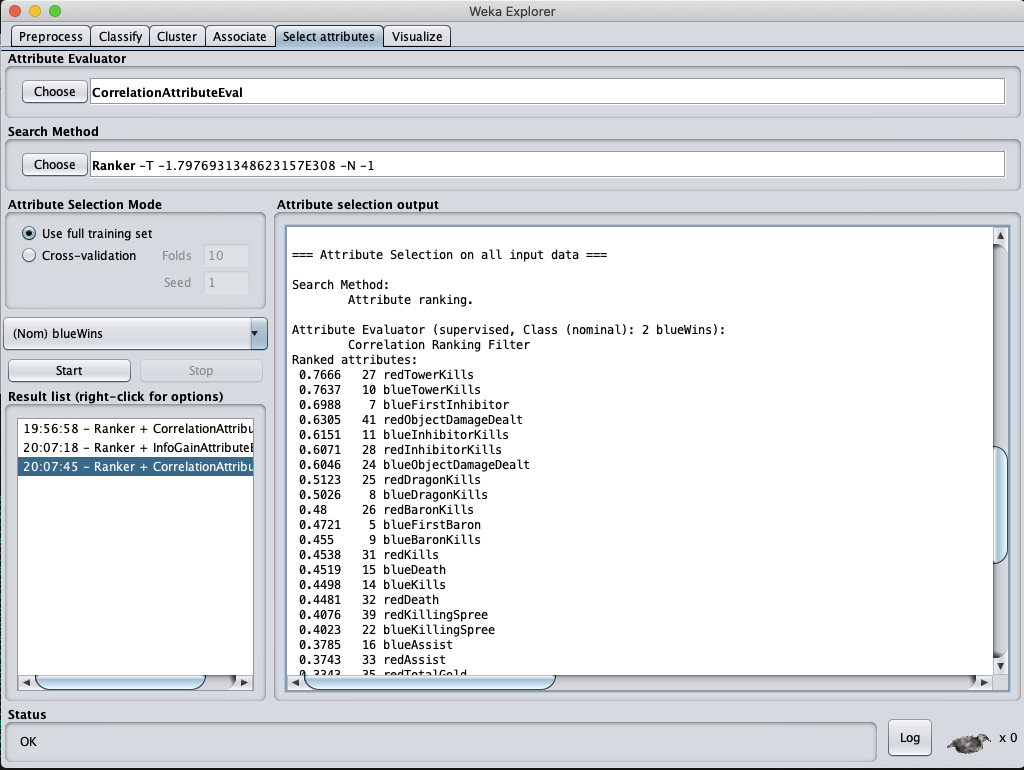
\includegraphics[width=0.7\linewidth]{graphs/weka_feature_selection.png}

\subsubsection{Two most importance feature graph}

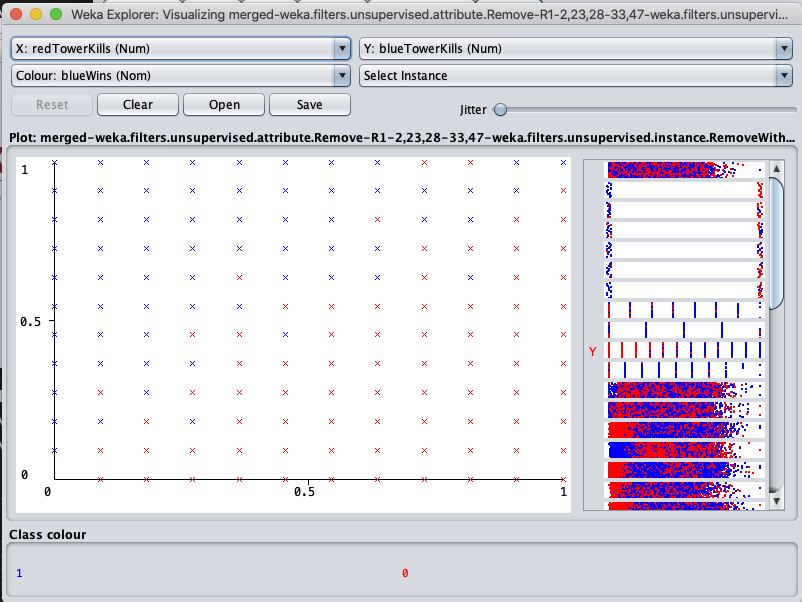
\includegraphics[width=0.7\linewidth]{graphs/weka_feature_graph_most_important_2.png}

\medskip

\subsection{Result}



Before Data preprocessing section we had 50 columns of dataset. We have examined every column. 
After we have applied the data preprocessing techniques, we reduced features to 40 without losing any information. 
\pagebreak



\section{Linear Classification}

In this section, we used Linear Classification to our dataset. Linear Classification helps us to classify the data by true/false or 1 and 0. as blueWins and redWins.


\subsection{Perceptron}


In data mining, Perceptron is the sensor for an algorithm to the supervised learning of binary classifiers.

\medskip

A binary classifier is a function that can decide whether an input represented by a vector of numbers belongs to a particular class.

\subsubsection{Performance Analyse}

We run like 5 times perceptron model with default parameters for get average values you can inspect below table for result.

\begin{table}[H]
\centering
\begin{tabular}{|cccc|}
\hline
\multicolumn{4}{|c|}{\textbf{Linear Classification: Perceptron Results}} \\ \hline
\#          & Training Time (ms)     & Error (cost)     & Score (\%)     \\ \hline
1           & 341.68                 & 0.018723         & 0.9813         \\
2           & 326.62                 & 0.018723         & 0.9813         \\
3           & 336.92                 & 0.018723         & 0.9813         \\
4           & 332.29                 & 0.018723         & 0.9813         \\
5           & 323.27                 & 0.018723         & 0.9813         \\ \hline
Average     & 332.16                 & 0.018723         & 0.9813         \\ \hline
\end{tabular}
\end{table}


\subsubsection{Feature Weight Analyse}

In this section, we inspect Perceptron instancee with coef\_ attribute (thanks to sckit-learn). with coef values we can get weights from first layer, so we applied this values with column features. there are some negative and positive values. Positive ones are most effective for class 1 (means blue win). Negative ones are most effective for class 0 (means red wins). According to this model, 3 Significant factor for class 0 are RedTotalLevel, redTotalGold, redTotalMinionKill. for class 1, BlueTotalLevel, blueTotalGold, blueTotalMinionKill. When we search on internet for these parameters, there are really effective for winnings. So each proffessional team is traning their players for improvements these features. You can inspect graph before.

\bigskip


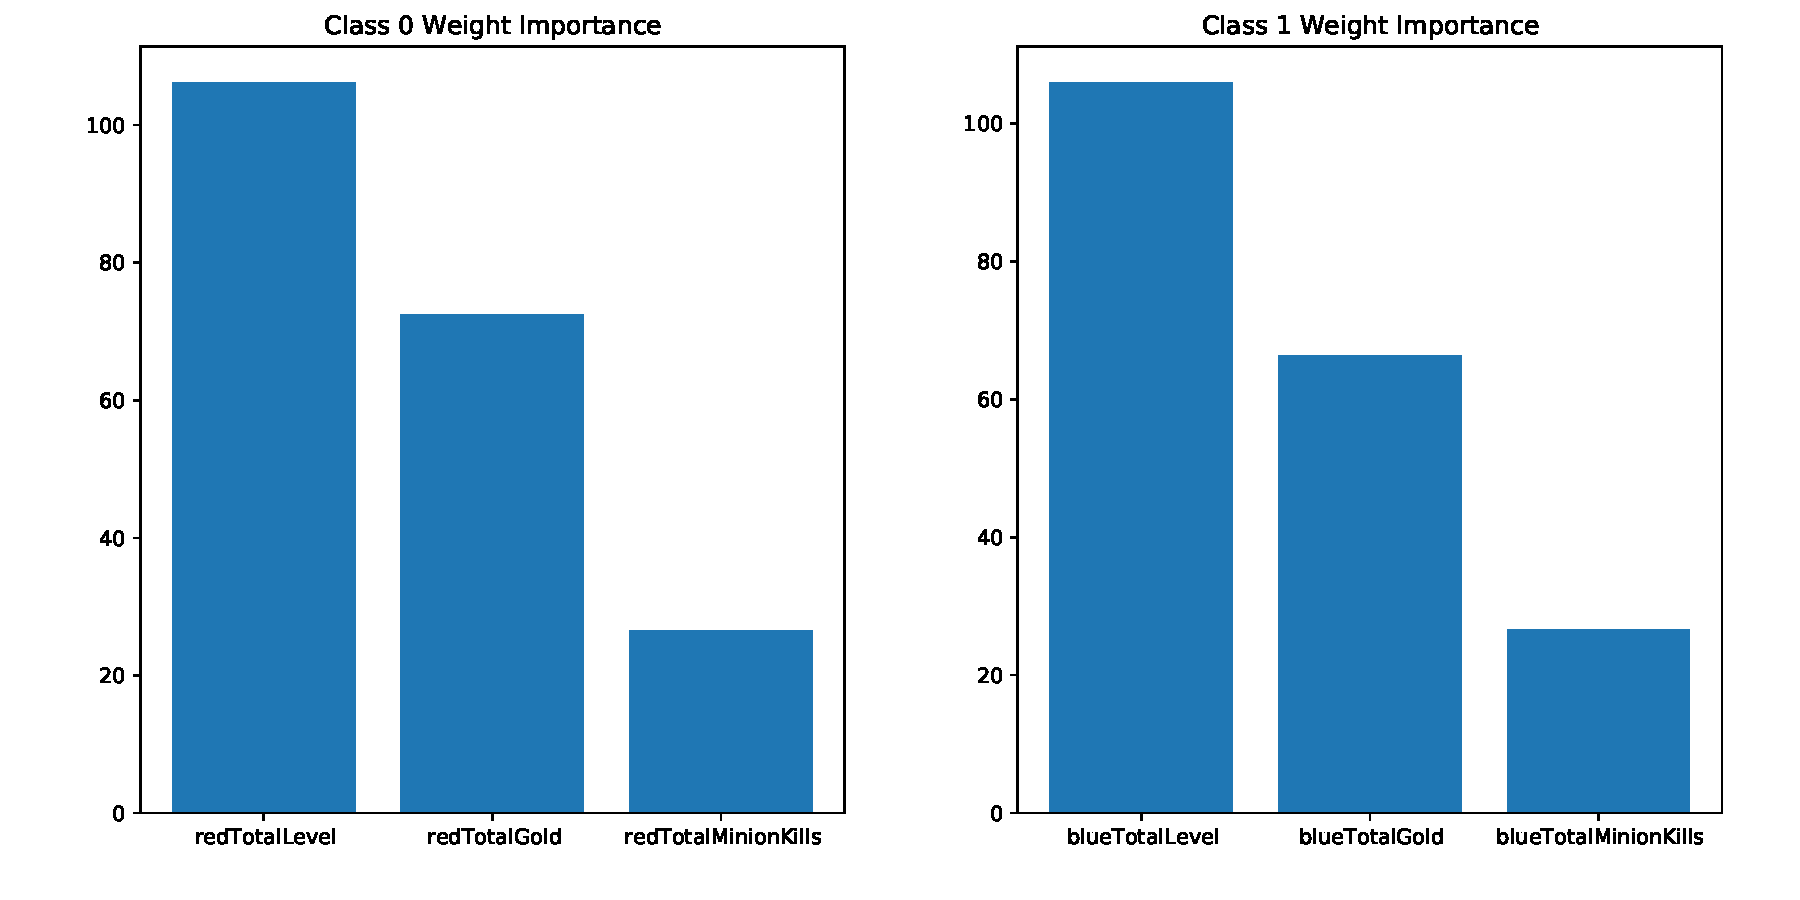
\includegraphics[width=.9\linewidth]{graphs/perceptron_feature_importance_weights.pdf}

\pagebreak

\subsubsection{Feature Analyse with BruteForce}

In this section, we analyze all values with randomly suffling, and these values are calculated to model-feature relation. when we suffle a feature, we look the model score, when its drop dramaticly. we decide to this feautre is important than others. These values very close to Feature Weight Analyse.

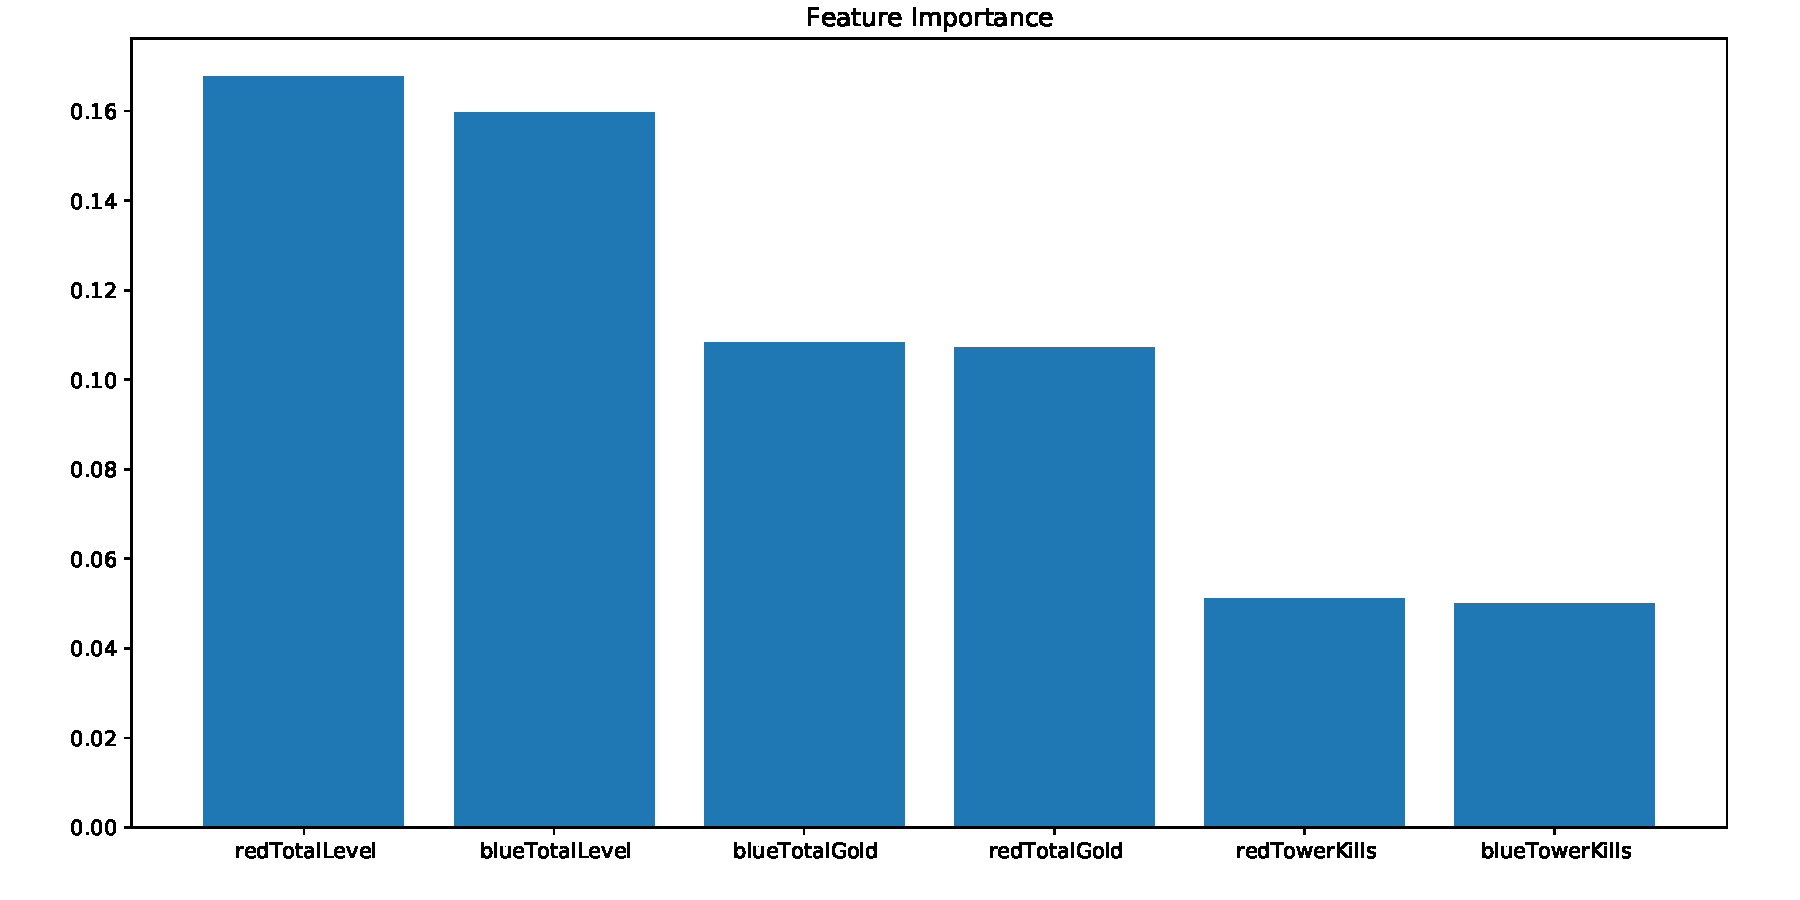
\includegraphics[width=.9\linewidth]{graphs/perceptron_feature_importance.pdf}


\subsubsection{Decision Boundary Graph}

We draw graph to with two importance features (according to model) and we draw line from first layer. You can inspect result below.

\medskip

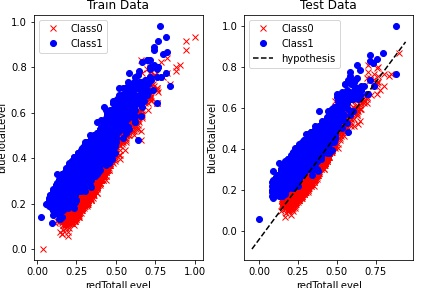
\includegraphics[width=.9\linewidth]{graphs/perceptron_decision_boundary.jpeg}


\pagebreak

\subsection{Logistic Regression}

Logistic regression is a statistical method used to analyze a data set with one or more independent variables that determine a result. The result is measured by a binary variable. In logistic regression, the dependent variable contains data coded as binary or binary, i.e. only 1 or 0. The purpose of logistic regression is to find the most suitable model to describe the relationship between a two-way characteristic and a set of independent variables. Logistic regression generates the coefficients of a formula to estimate the probability of the existence of the characteristics of interest for the transformation.

\subsubsection{Performance Analyse}

We run like 5 times  for get average values you can inspect below table for result.

\begin{table}[H]
\centering
\begin{tabular}{|cccc|}
\hline
\multicolumn{4}{|c|}{\textbf{Linear Classification : LogisticRegression Results}} \\ \hline
\#             & Training Time (ms)       & Error (cost)       & Score (\%)       \\ \hline
1              & 2048.80                  & 0.014602           & 0.9854           \\
2              & 2056.79                  & 0.014602           & 0.9854           \\
3              & 1871.26                  & 0.014602           & 0.9854           \\
4              & 2162.40                  & 0.014602           & 0.9854           \\
5              & 2640.21                  & 0.014602           & 0.9854           \\ \hline
Average        & 2155.89                  & 0.014602           & 0.9854           \\ \hline
\end{tabular}
\end{table}

\subsubsection{Feature Weight Analyse}

In this section, we applied same technique which we used before. According to this model, 3 Significant factor for class 0 are RedTotalLevel, redTotalGold, redTotalMinionKill. for class 1, BlueTotalLevel, blueTotalGold, blueTotalMinionKill. Which like we mentioned before, These values are very important. You can inspect Perceptron Model Section and below graphs.

\medskip

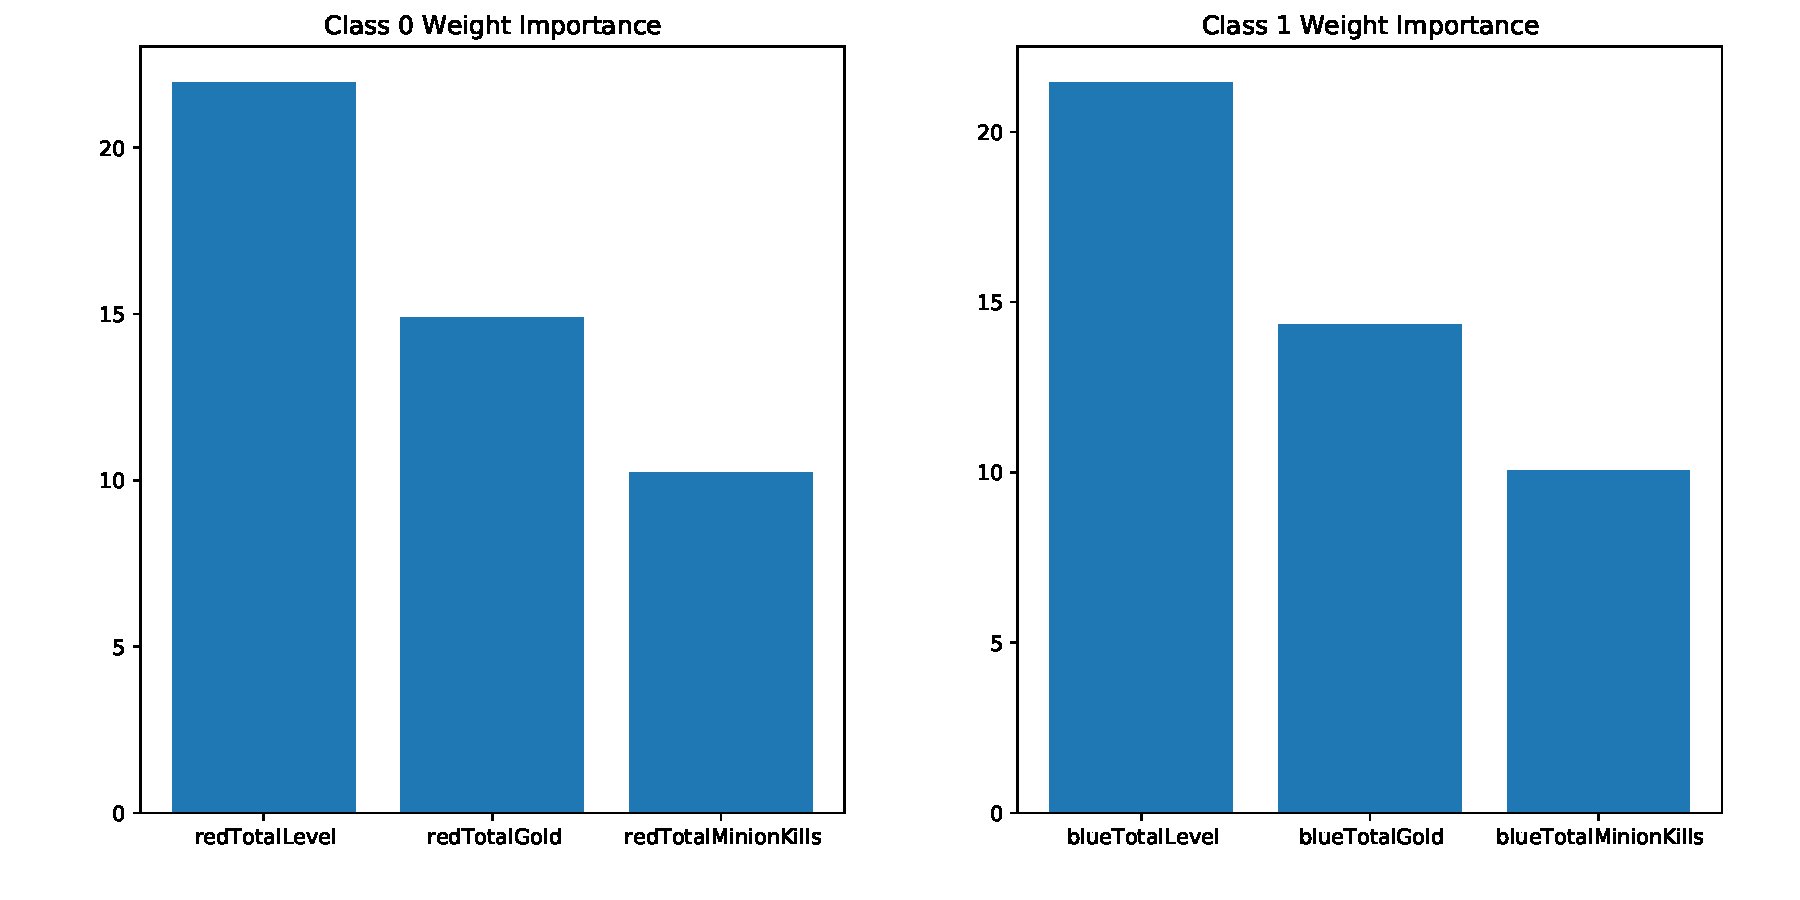
\includegraphics[width=.9\linewidth]{graphs/logisticregression_feature_importance_weights.pdf}

\pagebreak
\subsubsection{Feature Analyse with BruteForce}

In this section, we analyze all values with randomly suffling, and these values are calculated to model-feature relation. when we suffle a feature, we look the model score, when its drop dramaticly. we decide to this feautre is important than others. These values very close to Feature Weight Analyse except that we realized here two new paramters which do not mentioned above, blueTowerKill and redTowerkill these values are very familiar from weka Feature Analyse.

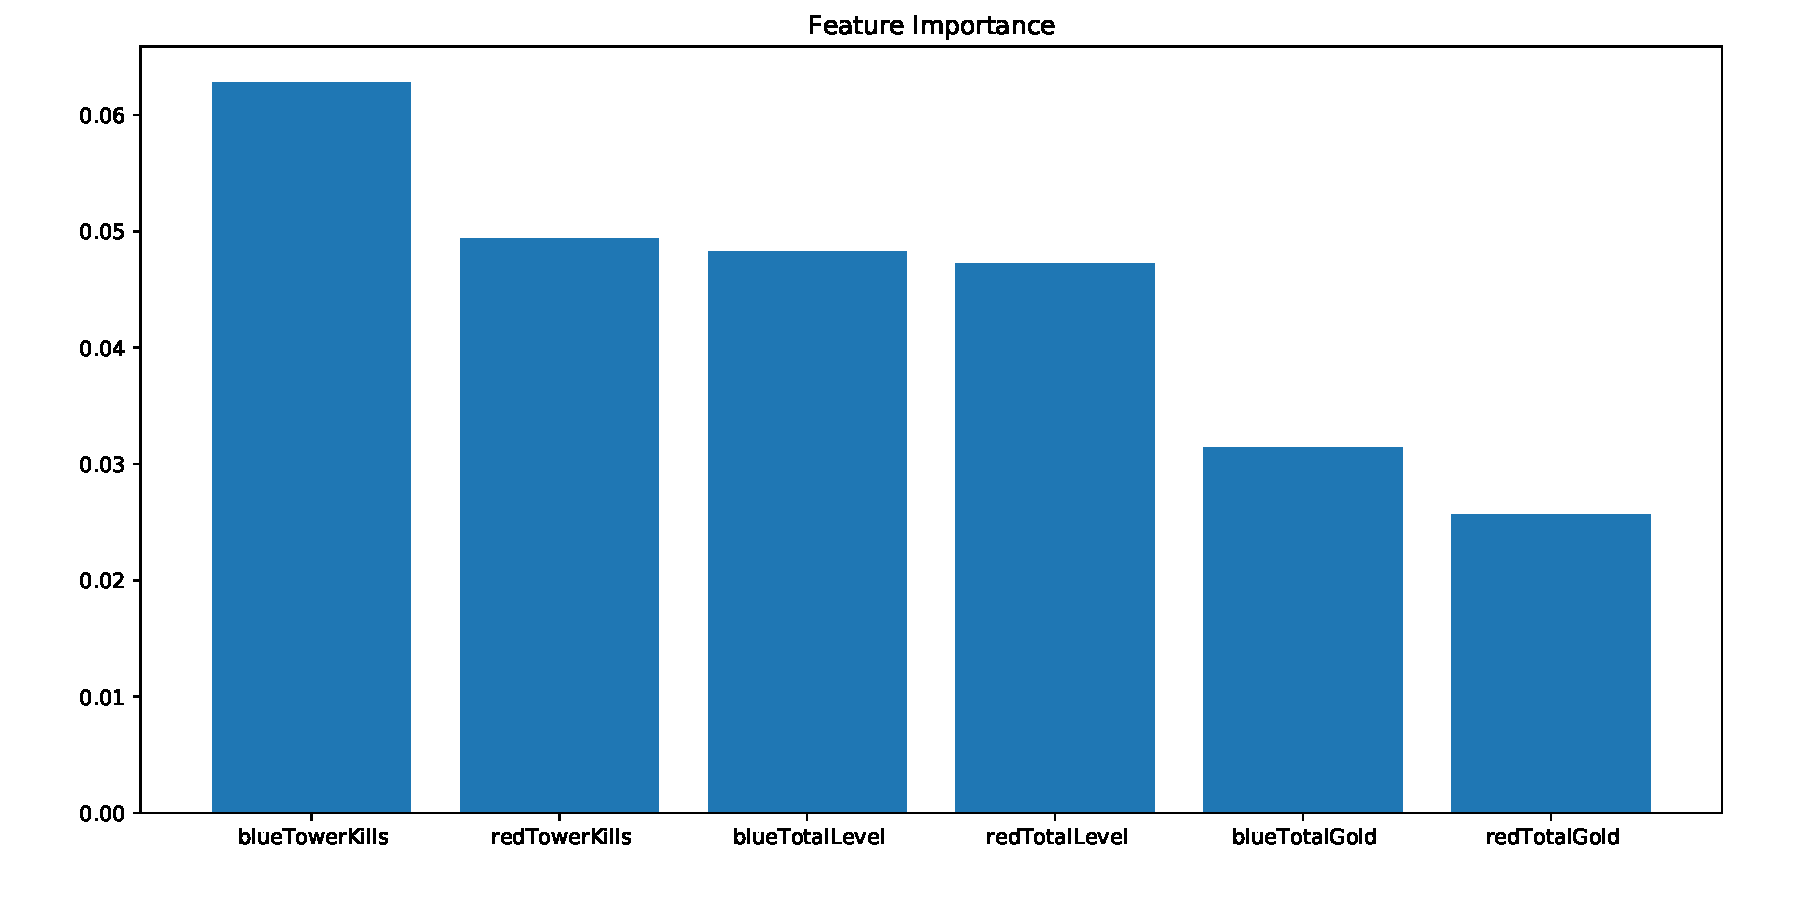
\includegraphics[width=.9\linewidth]{graphs/logisticregression_feature_importance.pdf}

\subsubsection{Decision Boundary Graph}

We draw graph to with two importance features (according to model) and we draw line from first layer. You can inspect result below.

\medskip

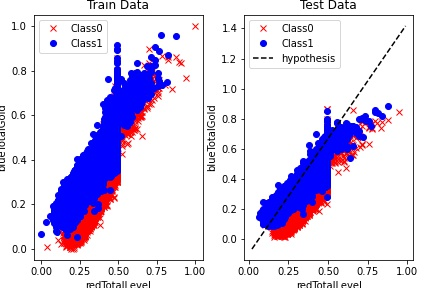
\includegraphics[width=.9\linewidth]{graphs/logisticregression_decision_boundary.jpeg}

\pagebreak

\subsection{SGD Classifier}

Stochastic Gradient Descent shorten as SGD is very effective function for the learning of linear classifiers under loss functions such as Support Vector Machines and Logistic Regression. While SGD has been around for a long time in the data mining space, it has recently became popular in the of large-scale learning.

\subsubsection{Performance Analyse}

We run like 5 times  for get average values you can inspect below table for result.

\begin{table}[H]
\centering
\begin{tabular}{|cccc|}
\hline
\multicolumn{4}{|c|}{\textbf{Linear Classification : SGDClassifier Results}} \\ \hline
\#           & Training Time (ms)      & Error (cost)      & Score (\%)      \\ \hline
1            & 211.66                  & 0.017651          & 0.9823          \\
2            & 203.04                  & 0.017342          & 0.9827          \\
3            & 215.69                  & 0.017365          & 0.9826          \\
4            & 218.15                  & 0.018128          & 0.9819          \\
5            & 202.84                  & 0.017532          & 0.9825          \\ \hline
Average      & 210.27                  & 0.017604          & 0.9824          \\ \hline
\end{tabular}
\end{table}

\subsubsection{Feature Weight Analyse}

In this section, we applied same technique which we used before. According to this model, 3 Significant factor for class 0 are RedTotalLevel, redTotalGold, redTotalMinionKill. for class 1, BlueTotalLevel, blueTotalGold, blueTotalMinionKill. Which like we mentioned before, These values are very important. You can inspect Perceptron Model Section and below graphs.

\medskip

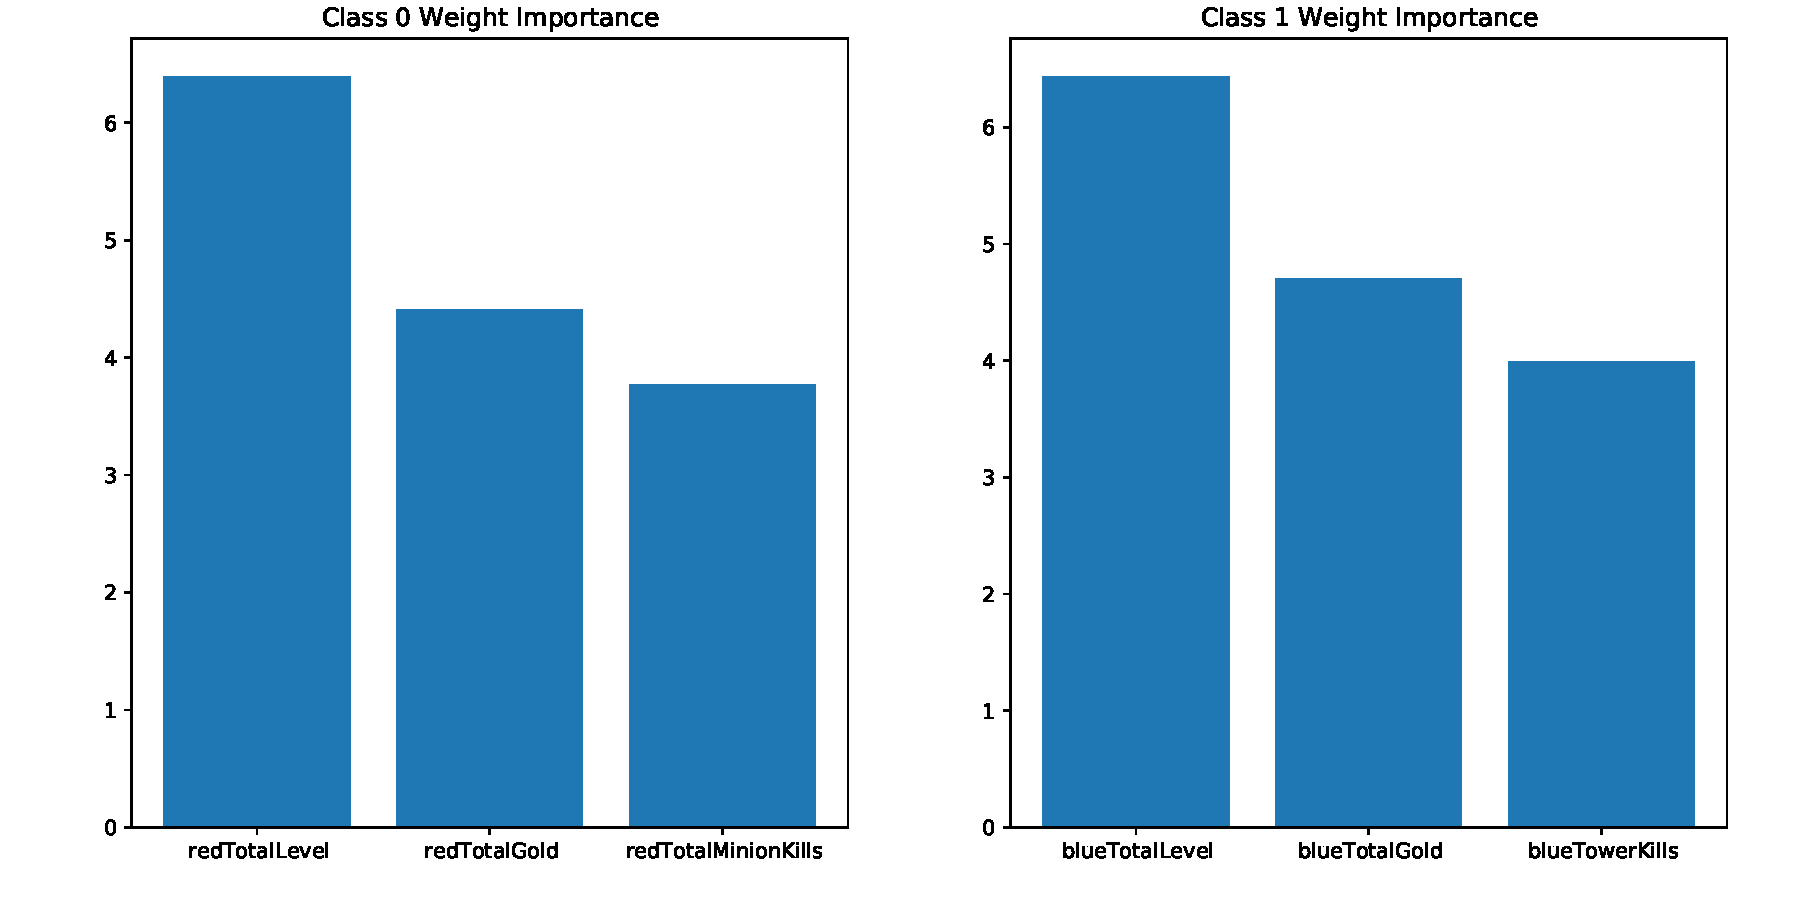
\includegraphics[width=.9\linewidth]{graphs/sgdclassifier_feature_importance_weights.pdf}

\pagebreak

\subsubsection{Feature Analyse with BruteForce}

In this section, we analyze all values with randomly suffling, and these values are calculated to model-feature relation. when we suffle a feature, we look the model score, when its drop dramaticly. we decide to this feautre is important than others. These values very close to Feature Weight Analyse except that we realized here two new paramters which do not mentioned above, blueTowerKill and redTowerkill these values are very familiar from weka Feature Analyse. (same like in LogisticRegression)

\medskip

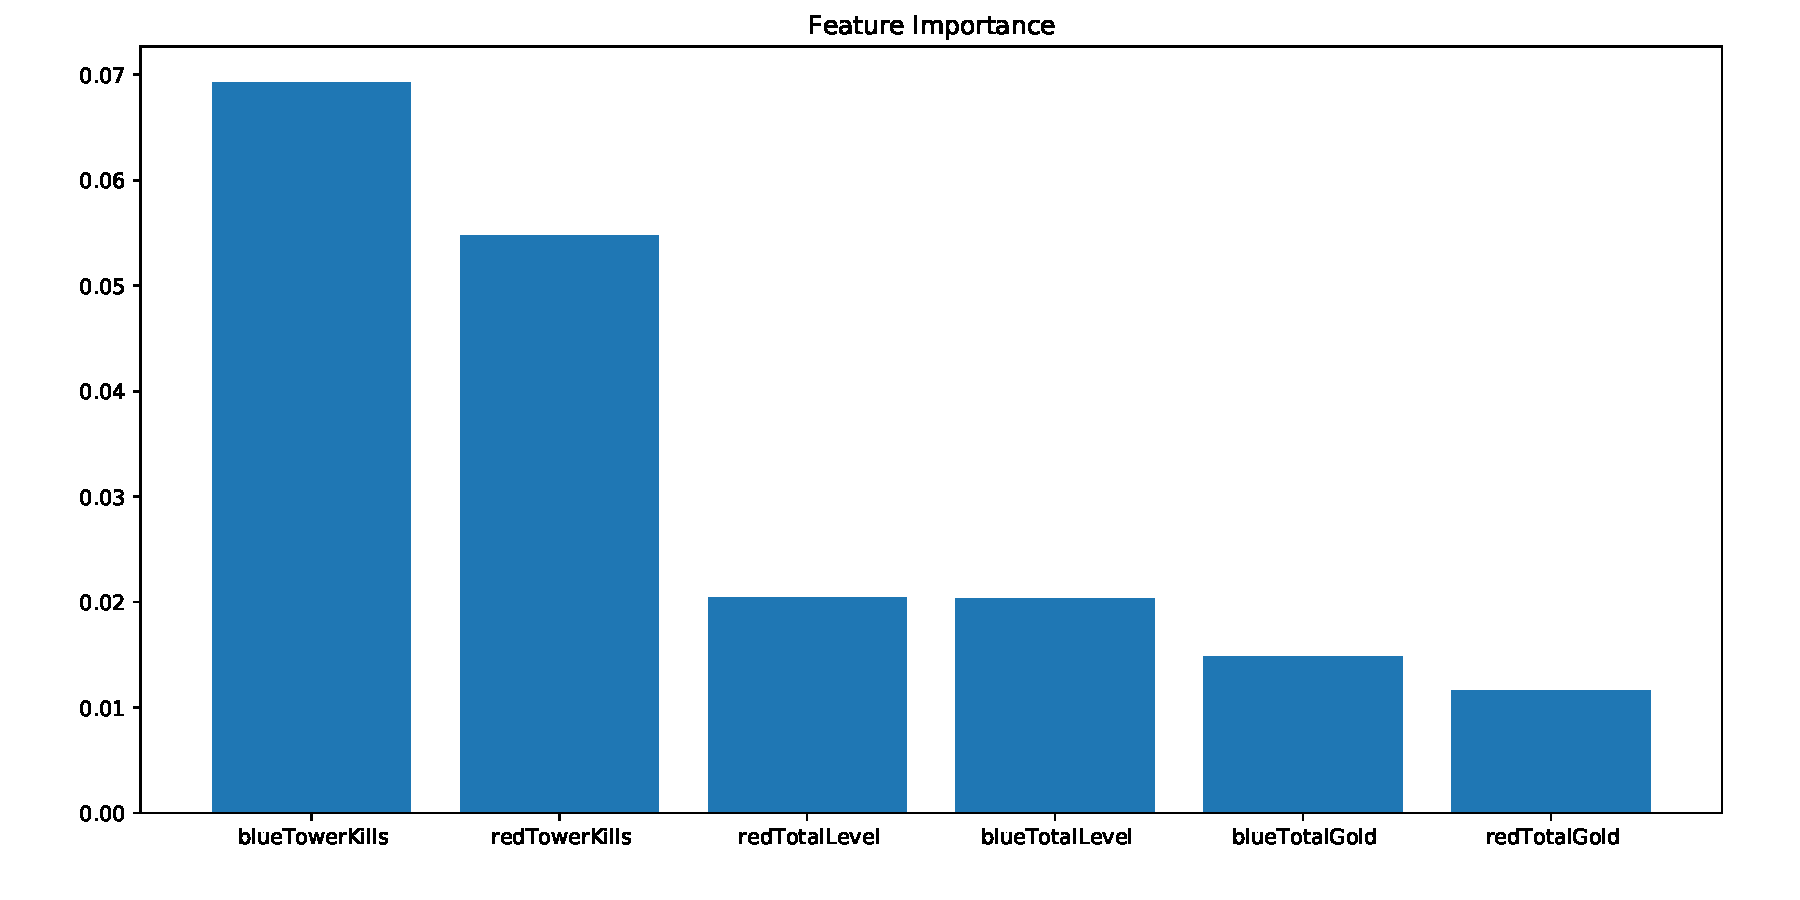
\includegraphics[width=.9\linewidth]{graphs/sgdclassifier_feature_importance.pdf}

\subsubsection{Decision Boundary Graph}

We draw graph to with two importance features (according to model) and we draw line from first layer. You can inspect result below.

\medskip

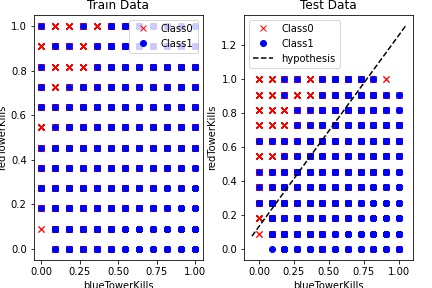
\includegraphics[width=.9\linewidth]{graphs/sgdclassifier_decision_boundary.jpeg}


\bigskip 

\pagebreak

\section{ Neural Network-based Classification}

\subsection{MLPClassifier}

There are many machine learning models available today. Neural Network is a machine learning model. It is a model inspired by the human brain and nervous system. We can also consider it as a Multi-layer Perceptron classifier. Neural Network is a structure in the form of layers. The first layer is called input and the last layer is called exit. The layers in the middle are called "Hidden Layers". Its layer contains a certain deemed 'Neuron'. These neurons are connected by "Synapse". Synapses contain a coefficient. These coefficients tell how important the information in the neuron to which it is attached is. Synapse Coefficients The value of a neuron is found by multiplying the inputs to that neuron by the coefficients and adding them together. This result found is put into an activation. According to the result from the function, it is decided that that neuron will not fire.


\subsubsection{Performance Analyse}

We run like 5 times  for get average values you can inspect below table for result. Compared to other models, it took longer than before. Also score's are higher than before.

\begin{table}[H]
\centering
\begin{tabular}{|cccc|}
\hline
\multicolumn{4}{|c|}{\textbf{Neural Network-based Classification : MLPClassifier Results}} \\ \hline
\#               & Training Time (ms)          & Error (cost)         & Score (\%)         \\ \hline
1                & 78774.47                    & 0.008028             & 0.9920             \\
2                & 50935.68                    & 0.008814             & 0.9912             \\
3                & 100431.51                   & 0.008385             & 0.9916             \\
4                & 62506.91                    & 0.009552             & 0.9904             \\
5                & 93354.18                    & 0.008028             & 0.9920             \\ \hline
Average          & 77200.55                    & 0.008561             & 0.9914             \\ \hline
\end{tabular}
\end{table}

\subsubsection{Feature Weight Analyse}

For this model manuel weight analyse is not possible, because there are a lot of layer and they are very complex like human brain. So we can not easily inspect this model so we do not have any data in this section.

\subsubsection{Feature Analyse with BruteForce}

for this model, this option is highly acceptable. like we mentioned before, in this technique we simply trying the brute-forcing. So this method we can figure out which features are very importants for our model.
You can inspect graph below.



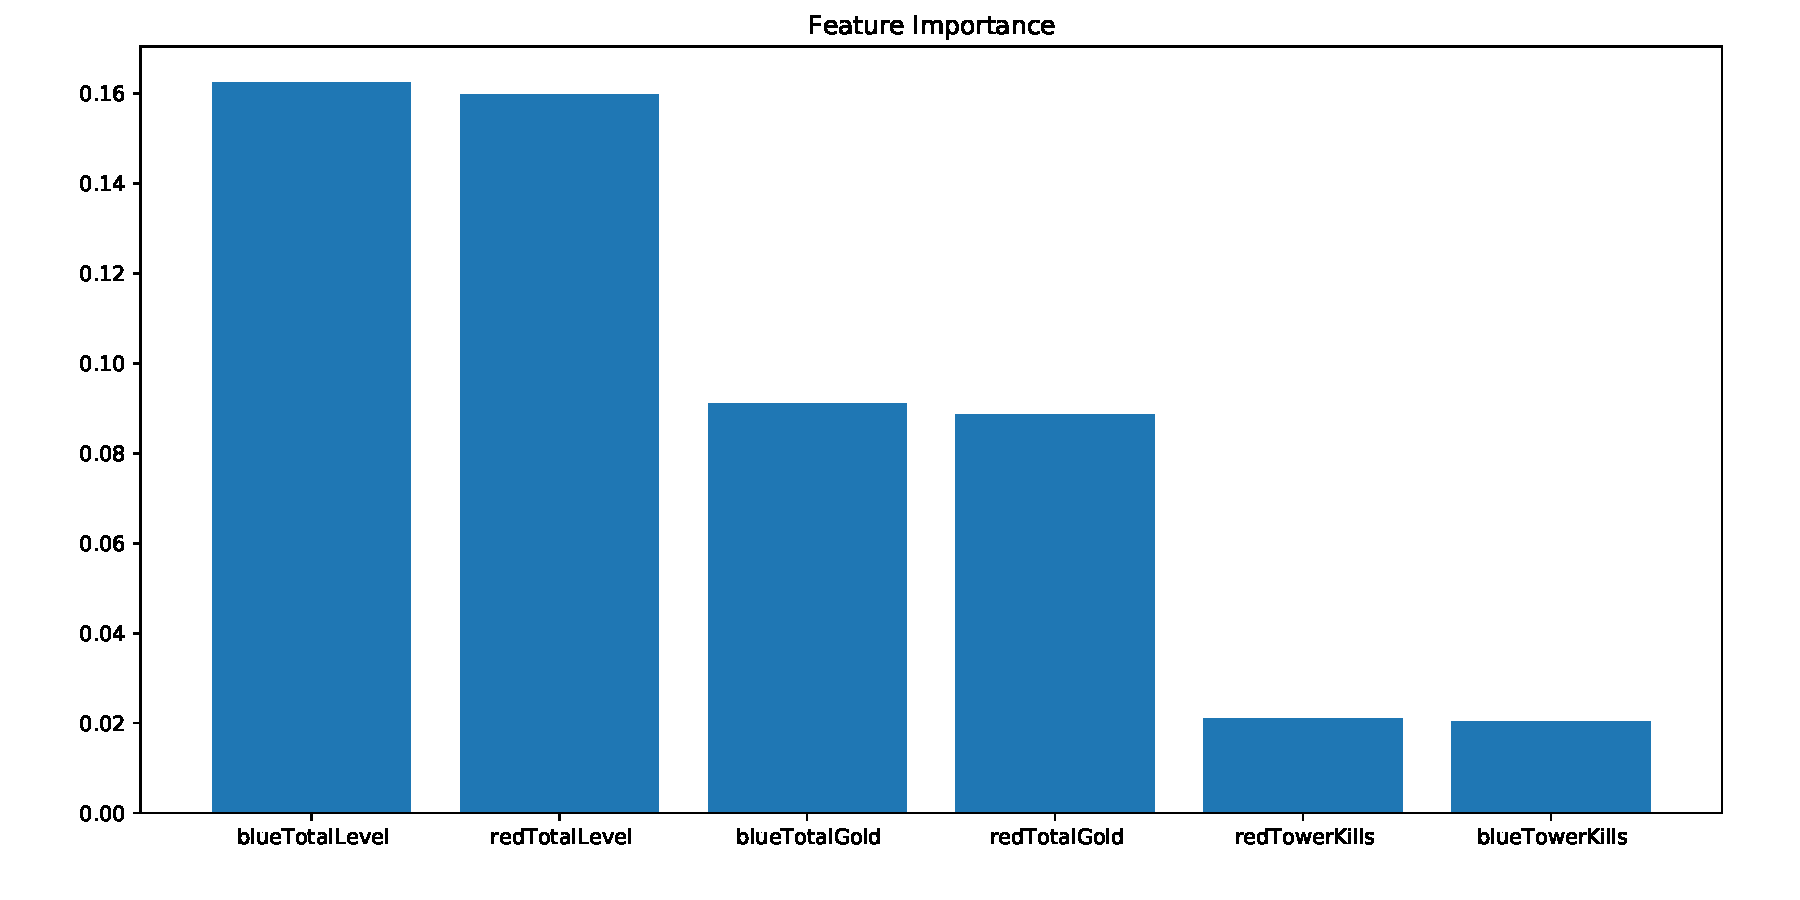
\includegraphics[width=.9\linewidth]{graphs/mlpclassifier_feature_importance.pdf}

\pagebreak

Also in this section we do not have decision boundary because of complexity bu we simply show the data values on 2d space. You can inspect graph below.

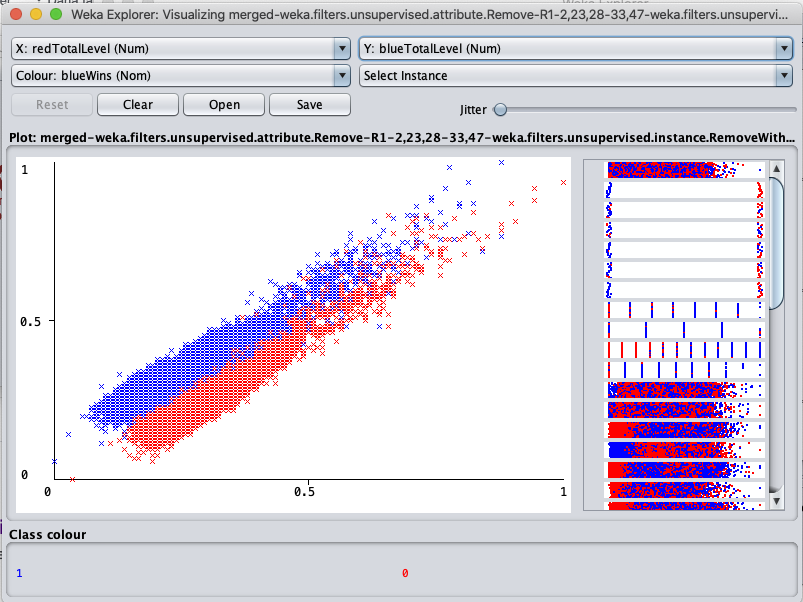
\includegraphics[width=.9\linewidth]{graphs/mlpclassifier_feature_graph.png} %TODO


\section{Clustering}

\subsection{KMeans}

Clustering is the division into groups that show similar characteristics in a data set. There are many similarities within the same cluster and fewer similarities between clusters. There is Unsupervised Learning, meaning no prior information is given. K-Means and Hierarchical Segmentation are among the commonly used clustering algorithms. These algorithms are frequently used such as customer segmentation, market segmentation, and computer vision.
\medskip

\subsubsection{Performance Analyse}

We run like 5 times  for get average values you can inspect below table for result. Compared to other models, it have worst accurracy, after some research we decide to our dataset not compatible for clustering. You can look feature importance and step by step clustering graphs below.



\begin{table}[H]
\centering
\begin{tabular}{|cccc|}
\hline
\multicolumn{4}{|c|}{\textbf{Clustering : KMeans Results}} \\ \hline
\#       & Training Time (ms) & Error (cost) & Score (\%)  \\ \hline
1        & 530.31             & 0.123487     & -57026.2996 \\
2        & 518.64             & 0.876560     & -57026.2900 \\
3        & 545.30             & 0.876346     & -57026.2258 \\
4        & 518.68             & 0.876536     & -57026.2771 \\
5        & 522.59             & 0.123464     & -57026.2112 \\ \hline
Average  & 527.10             & 0.575279     & -57026.2607 \\ \hline
\end{tabular}
\end{table}

\subsubsection{Feature Importance with BruteForce}
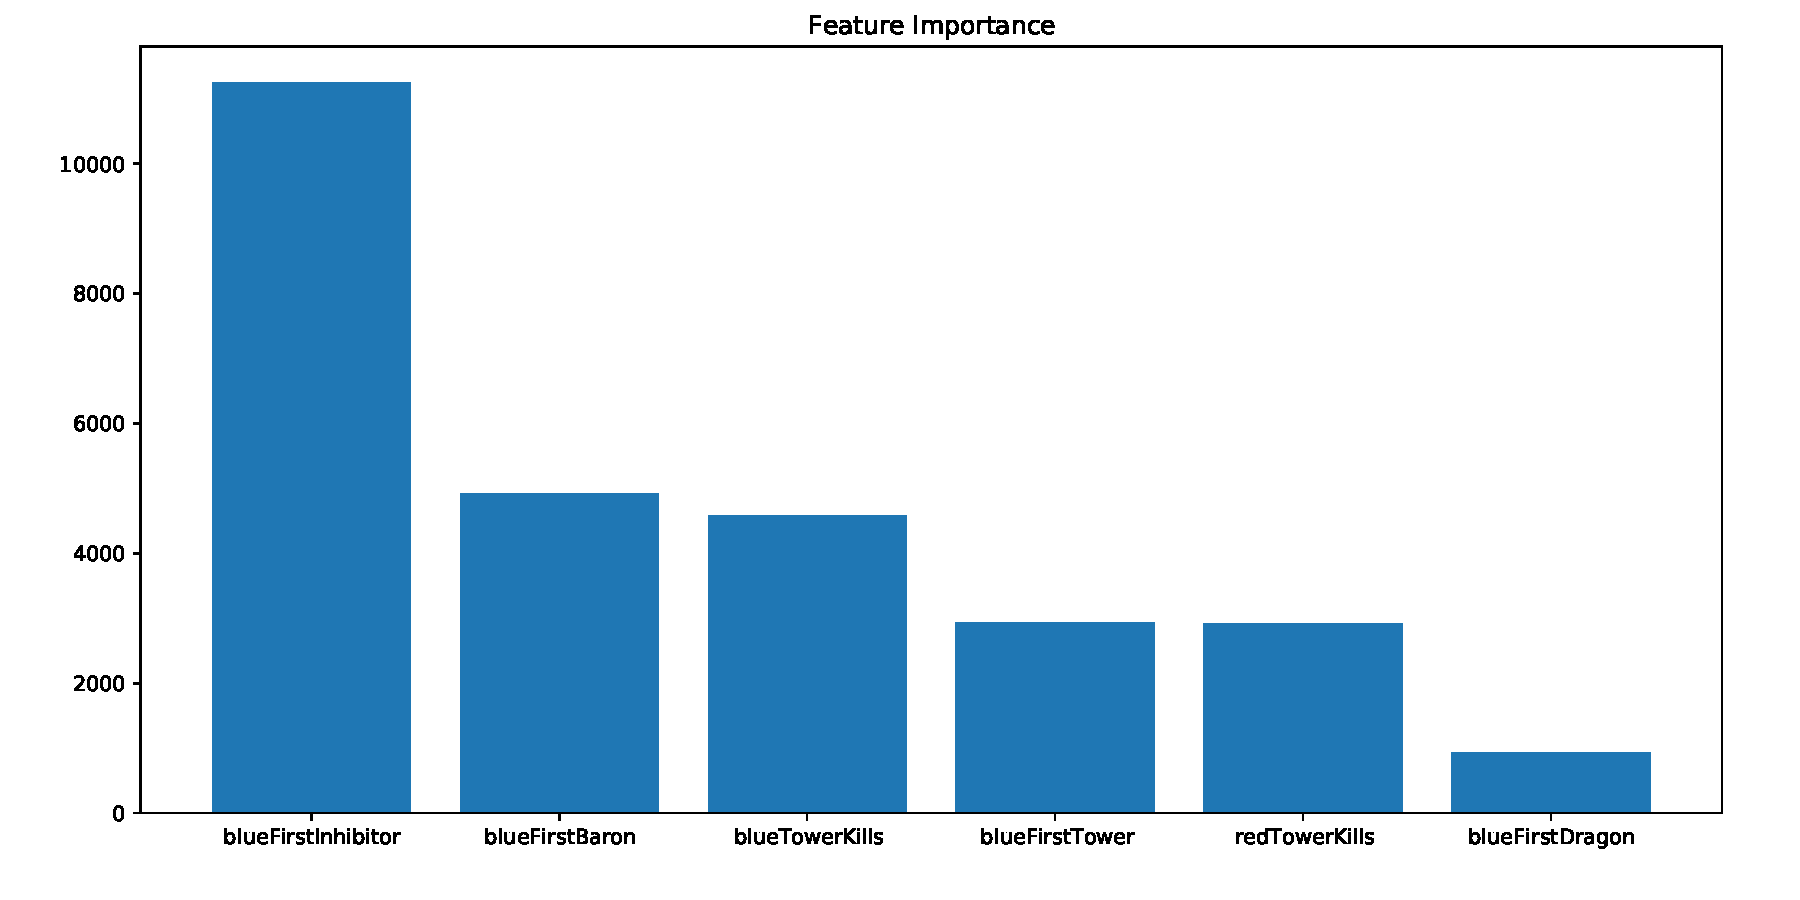
\includegraphics[width=.9\linewidth]{graphs/kmeans_feature_importance.pdf}

\medskip

\subsubsection{Clustering Step by Step}
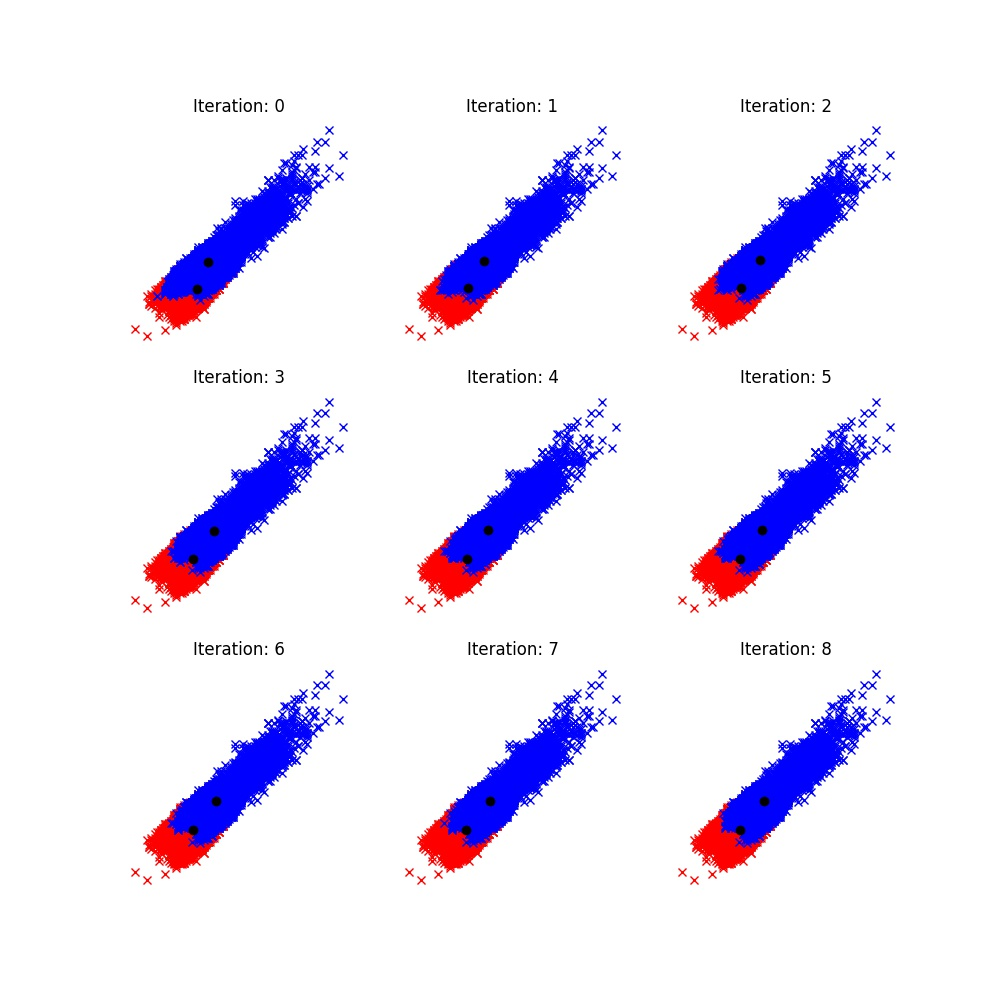
\includegraphics[width=.9\linewidth]{graphs/kmeans_clustering_progress.jpeg}


\pagebreak

\textsc{\LARGE \bf Conclusion}\\
\medskip

As a conclusion, In this project we experience a lot of different technique and models as a team. We research this problem under 4 main topic and we use 8 different tool and model. Each model select almos same parameters and scores. We get to best result with mlpclassifier. Also clustering section we get worst results and we can not easily fix this, after some research we decide to our dataset not compatible with clustering. In this assigment we learned debug and know how to about models.
%------------------------------------------------

\end{document}
